\textit{Breve recap}.

I telescopi sono strumenti in grado di raccogliere i fotoni che arrivano distribuiti nello spazio in un punto detto "fuoco" (di un'ottica che può essere sia un rifrattore che un riflettore) e sono in grado di aumentare la nostra capacità di vedere oggetti angolarmente piccoli.

Abbiamo visto che la capacità di raccogliere fotoni va con l'apertura (diametro) del telescopio al quadrato ($D^2$), mentre il potere risolutivo va con il diametro.

Abbiamo visto che i telescopi, in quanto oggetti fisici, sono soggetti ai difetti tipici dell'ottica: alcuni sono legati alla forma (che quindi può essere quantomeno corretta); altri, come il coma, sono invece semplicemente legati al fatto che possono osservare in maniera ottimale ciò che è sull'asse del telescopio, ma magari hanno dei difetti quando si guardano oggetti fuori dall'asse del telescopio. Ma qual è la grandezza dei difetti di cui parliamo?

\begin{figure}[H]
    \centering
    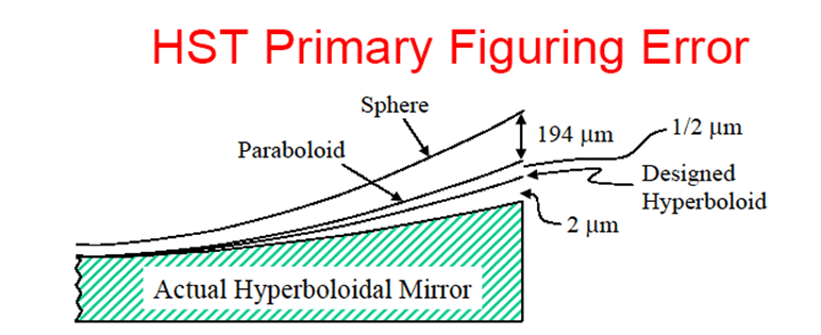
\includegraphics[width=8cm]{immagini/errore_space_telescope.png}
\end{figure}

Per dare un'idea di quali numeri sono in gioco, quando volò lo Space Telescope ci fu un problema poiché le immagini non avevano la qualità ottica desiderata: in pratica lo specchio dello Space Telescope, che è dell'ordine di 2,5 metri, era stato lavorato male e quindi non vedeva così bene come si voleva. Fu fatta una missione spaziale per correggere questo difetto ottico. Abbiamo detto che il telescopio dovrebbe essere più una parabola: questa parabola era sostanzialmente 2,5 $\rm \mu m$ più schiacciata di quella che avrebbe dovuto essere, quindi un errore tale porta ad una immagine di qualità non utile per l'osservazione (questo ci dà un'idea su quanto si deve essere precisi nel fare i disegni e con che precisione bisogna lavorare per l'ottica).

\vspace{0.2cm}Stiamo studiando i riflettori, i quali prevedono che i raggi provenienti dalla sorgente convergano nel fuoco che prende il nome di "primo fuoco".

In telescopi di questo genere, il primo fuoco del telescopio, che si trova tra la sorgente e lo specchio, deve essere occupato da uno strumento:

\begin{figure}[H]
    \centering
    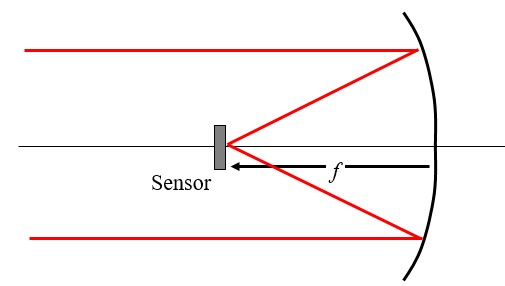
\includegraphics[width=9cm]{1.jpg}
\end{figure}

Qui, al primo fuoco, è stato sospeso uno strumento sul quale si posizionavano delle lastre fotografiche. Tale strumento (come ad esempio quello del telescopio di Monte Palomar) è abbastanza grande da contenere un operatore\footnote{Per i bimbi di Siringo: si intende un uomo che posiziona le lastre fotografiche, non una matrice unitaria.}.

Questo tipo di configurazione ottica non è ottimale, per il semplice motivo che non si può avere uno strumento di misura molto grande (se ad esempio abbiamo un telescopio di 1 metro, come quello di Serra La Nave, e ci posizioniamo, questo strumento non potrà essere allocato, perché farebbe ombra); inoltre se usassimo solo il primo fuoco avremmo una focale $f$ corta, cioè la distanza tra lo specchio e il fuoco non potrebbe essere ovviamente nulla, perché altrimenti lo strumento dovrebbe essere esteso (per esempio con uno specchio di 1 metro, difficilmente potremo avere una focale maggiore di 3 metri, altrimenti dovremmo costruire un telescopio alto come un palazzo e questo potrebbe avere altri tipi di problemi). Ricordiamo che la focale corta significa una proiezione sul piano focale molto piccola, in quanto l'immagine è proporzionale a $f \alpha$.

Entra allora in gioco la configurazione \textbf{Cassegrain Telescope}:

\begin{figure}[H]
        \centering
        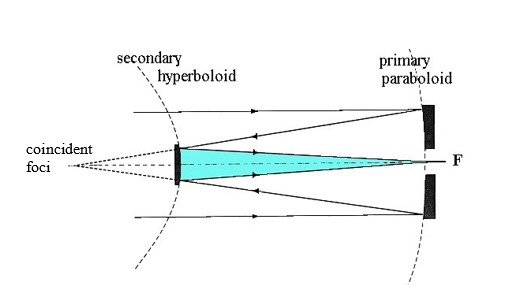
\includegraphics[width=9cm]{2.jpg}
    \end{figure}
\begin{figure}[H]
        \centering
        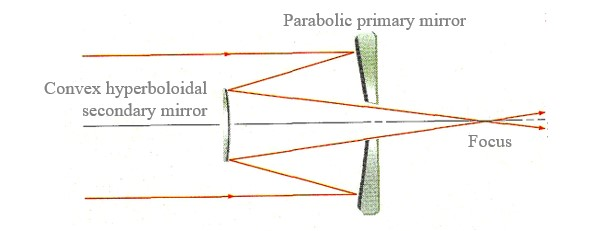
\includegraphics[width=9cm]{3.jpg}
    \end{figure}

L'idea è di sospendere uno specchio che prende il nome di \textit{specchio secondario} (il nome è dovuto all'ordine con cui vengono colpiti dai raggi), che nel Cassegrain Telescope è un iperboloide, per poter estrarre il fascio sotto il primario. A questo punto il primario può anche essere forato (perché tanto è in ombra del secondario).

Questa è la configurazione con cui si costruiscono di fatto tutti i telescopi. I vantaggi di questa configurazione sono ovvi: l'oggetto più pesante, che è lo specchio, sta sotto, può avere montato lo strumento (lo strumento può essere grande quanto si vuole, anche molto più grande del telescopio stesso perché non impedisce alla radiazione di raggiungere il primario). Un vantaggio ulteriore di una configurazione di questo genere è che quando c'è un coma si manifesta elongato in una direzione sul primario ed elongato nella direzione opposta sul secondario, di conseguenza si compensano e questi sistemi permettono di avere una qualità ottica migliore. In più si può avere una lunga focale perché, se ricordiamo dall'ottica che la focale complessiva di un sistema ottico è data da

$$\frac{1}{f} = \frac{1}{f_1} + \frac{1}{f_2}$$

possiamo avere focali molto estese in una configurazione meccanicamente molto compatta (ad esempio a Serra La Nave c'è un telescopio che ha una distanza tra il primario e il secondario che è dell'ordine di un paio di metri fisicamente, ma che ha una focale equivalente di 16 metri); dunque possiamo avere una grandissima focale (che, ricordiamo, riduce le aberrazioni perché vanno con il cubo della focale) in una struttura estremamente compatta.

Potremmo pensare che, mettendo un specchio dove dovrebbe essere il soggetto, non vediamo il soggetto. Non è così: gli oggetti da osservare sono così lontani che, pur essendo sorgente di onde sferiche, la luce prodotta ci arriva come un fascio piano, che si propaga lungo una sola direzione; questo è il motivo per cui due persone riescono a vedere la stessa stella (mentre per esempio, in un aula, mentre uno studente vede la porta, il prof. potrebbe non vederla perché messo in un punto in cui vede lo spigolo del muro e quindi c'è un problema di prospettiva: ciò perché la porta è vicina; se invece il prof. e lo studente guardano qualcosa di lontano, il fatto che loro siano posti in due posizioni differenti, non pone questo problema di prospettiva, perché non stanno vedendo porzioni diverse del fronte d'onda, ma la medesima). Quindi il fatto che lo specchio sia al centro, rompe il fronte d'onda, ne diminuisce il numero di fotoni, ma non la direzione e quindi l'immagine.

Quindi, per concludere, ribadiamo che il Cassegrain Telescope è fatto da un parabolico e da un iperbolico. 

Poi c'è un'altra configurazione, che è quella di Serra La Nave, che prende il nome di “Ritchey - Chrétien” dove gli specchi sono due iperboloidi che compensano al meglio le aberrazioni tipiche delle ottiche.

\begin{figure}[H]
        \centering
        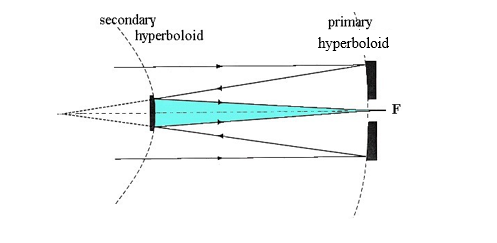
\includegraphics[width=10cm]{4.png}
    \end{figure}

Quindi, la maggior parte di tutti i telescopi è fatta, sostanzialmente, in questo modo.

Un po' diversi sono invece i telescopi chiamati “gregoriani”. 

\begin{figure}[H]
        \centering
        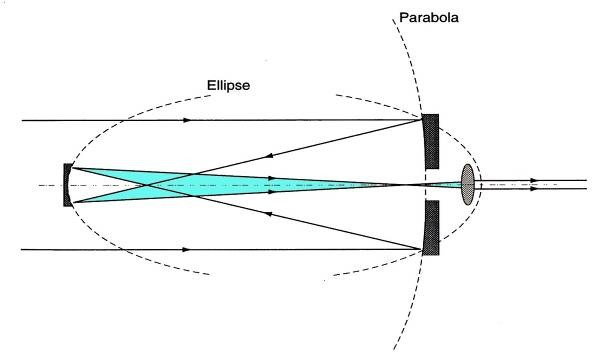
\includegraphics[width=10cm]{5.jpg}
        \label{}
    \end{figure}

Essi hanno il primario che è una parabola e il secondario che è una ellisse. Essendo coniche, perché siano allineate devono avere il medesimo asse di simmetria e devono avere i fuochi coincidenti (se così non fosse, il sistema non sarebbe allineato, non avrà il fuoco). Il telescopio gregoriano è tipico degli osservatori solari (e anche di qualche radiotelescopio), in quanto ha un fuoco intermedio. Ciò vuol dire che in linea di principio potremmo collocare un disco (vedi immagine), per esempio, con un foro per vedere una piccola porzione del Sole. Potremmo usare questo foro per ridurre la quantità di energia che dal Sole altrimenti arriverebbe sullo specchio (stiamo parlando di 1 $\rm kW/m^2$, con un telescopio di 4 metri ci ritroveremmo a dover dissipare una quantità di energia mostruosa, che possiamo dissipare tutta su questo diaframma dove facciamo passare un pezzetto di luce del Sole che dobbiamo guardare).

\subsubsection{Come è realizzato un telescopio}
Vediamo ora di cosa sono fatti i telescopi.

I telescopi sono fatti di vetro, reso riflettente da uno strato di un metallo (solitamente è alluminio) posto dietro.

Nonostante il vetro sia un oggetto pesantissimo, i telescopi sono realizzati con tale materiale perché ha un coefficiente di espansione basso (pari a $\rm 0,02 \cdot 10^{-7} \, K^-1$), ciò vuol dire che il telescopio mantiene la sua forma (ricordiamo che nella precedente sezione si parlava di $\rm \mu m$ di deformazione, che potrebbero essere dovuti a escursione termica). Il fatto che l'espansione termica sia di questo ordine di grandezza fa sì che una differenza di temperatura giorno-notte, inverno-estate (che può essere anche di 50°), è comunque tale da non cambiare la forma del telescopio. 

Per realizzare una lente si fonde il vetro e lo si pone in una vasca, la quale poi viene messa in rotazione; quando il vetro si raffredda si lavora per dargli la forma di iperboloidi, paraboloidi ecc. Il fatto che sia già in rotazione dà al vetro una forma che lo avvicina ad una parabola (notiamo che stiamo parlando, tra l'altro, di un oggetto che pesa 15 tonnellate).

\begin{figure}[H]
        \centering
        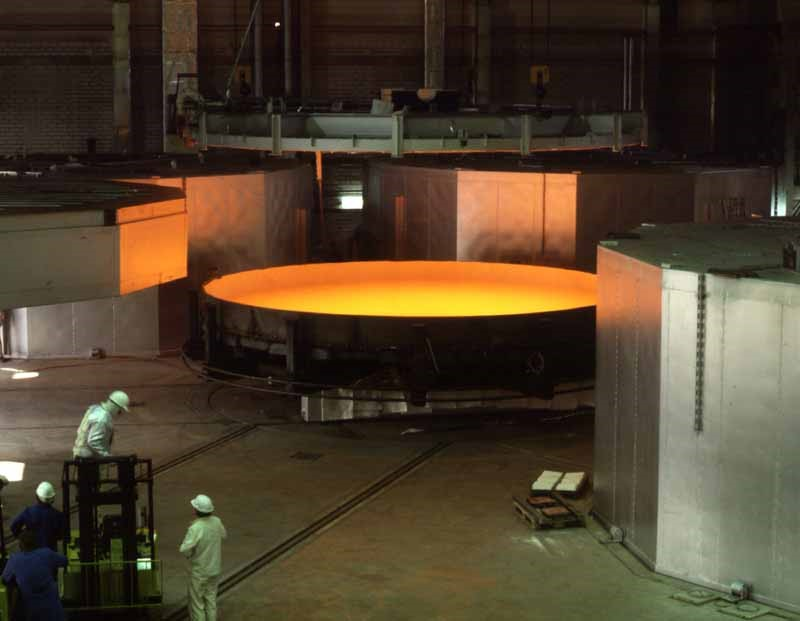
\includegraphics[width=7cm]{6.jpg}
        \label{}
\end{figure}

Questo è tecnicamente il limite di quelli che sono i telescopi costruiti con un solo specchio, quindi detti \textit{monolitici}. I telescopi più grandi vengono costruiti invece con un insieme di specchi esagonali che vengono assemblati per dare la forma che si vuole (un po' come il pallone da calcio, in cui con gli esagoni realizziamo una sfera). In figura si vede il telescopio del Keck, dove al centro vi è un foro in cui è posto l'operatore e da cui passa la luce.

\begin{figure}[H]
        \centering
        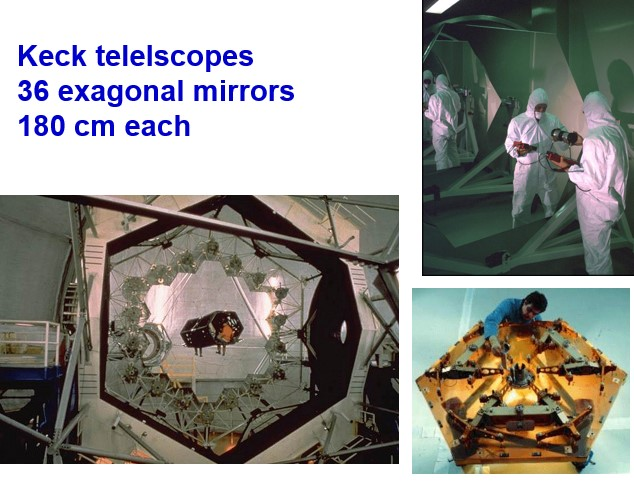
\includegraphics[width=7cm]{7.jpg}
\end{figure}

Un altro problema che si riscontra nella lavorazione di oggetti così imponenti è l'allineamento. Infatti il monolitico non ha soltanto il compito di raccogliere la luce, ma ha anche quello di spedire tutta la luce che arriva sul fuoco in fase, altrimenti non ha potere risolutivo (se non fosse così non sarebbe più una fenditura). Quindi il problema principale di questo dispositivo è che gli specchi devono essere messi in maniera tale che la loro distanza dallo specchio secondario sia esattamente un multiplo della lunghezza d'onda, altrimenti la radiazione non andrà più in fase. Se non sono in fase, quello che si otterrebbe è tanta luce, ma non si avrebbe potere risolutivo. Adesso vedremo come si risolvono questi problemi (il motivo per cui questi oggetti sono nati adesso è che adesso abbiamo una elettronica veloce, 20 anni fa non potevano funzionare o funzionavano male).

Mentre nel caso di specchio circolare la point spread function (che è una funzione che mostra come la luce si diffonde o si espande intorno a un punto luminoso ideale quando attraversa un sistema ottico) ha la forma del disco di Airy, nel caso di specchi esagonali la forma che si osserva per la luce emessa da una sorgente puntiforme è quella mostrata in figura:

\begin{figure}[H]
    \centering
    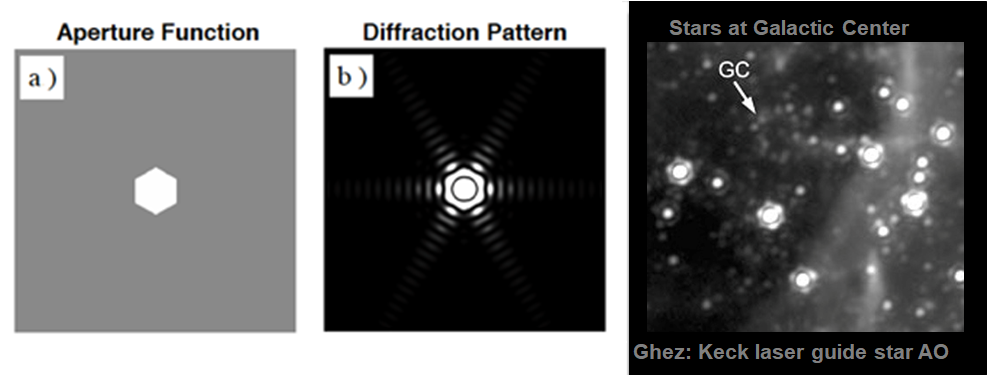
\includegraphics[width=10cm]{immagini/immagine_specchi_esagonali.png}
\end{figure}

\subsubsection{Montature e proprietà del telescopio}
Sorge un altro problema: noi osserviamo oggetti che, nel nostro sistema alto-azimutale, sorgono e tramontano. Bisogna allora inventare una meccanica che permetta di seguire l'oggetto. La prima meccanica realizzata con questo obiettivo è stata la cosiddetta \textit{montatura equatoriale}:

\begin{figure}[H]
        \centering
        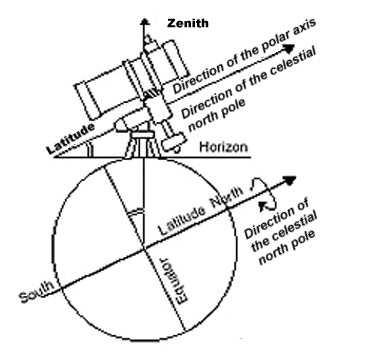
\includegraphics[width=7cm]{8.jpg}
\end{figure}

I telescopi sono stati montati su questa montatura in modo da non dovere "seguire" l'oggetto. Si immagina di avere un proprio orizzonte, una verticale che va verso lo zenit, e un'asse che è parallelo all'asse di rotazione terrestre. Così facendo il telescopio deve solo ruotare attorno a quest'asse per compensare l'asse di rotazione terrestre, quindi deve girare esattamente all'opposto con la velocità dell'orologio (per definizione). Questa è la montatura più diffusa ed è quella che abbiamo a Serra La Nave, e questo è un esempio di come si realizza (nella foto c'è uno dei telescopi di Serra La Nave quando era ancora in officina. Abbiamo una sorta di forcella che ruota per tenere il telescopio sempre puntato sull'oggetto che, questa volta, descrive un cerchio nel sistema equatoriale).

\begin{figure}[H]
        \centering
        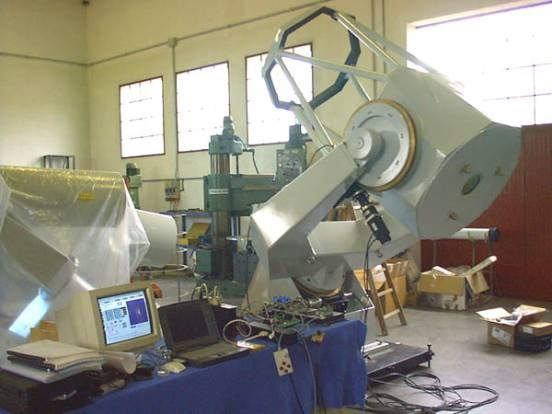
\includegraphics[width=9cm]{9.jpg}
\end{figure}

Si tratta di un telescopio piccolissimo, di 80 cm, ma con questa montatura si facevano anche telescopi grandi. Nell'immagine seguente, per esempio, vi è la montatura “Fork mount” di un telescopio di 3,6 metri dell'ESO.

\begin{figure}[H]
    \centering
    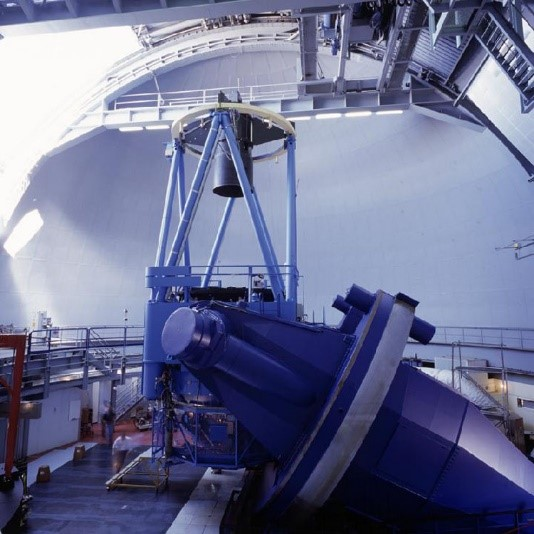
\includegraphics[width=9cm]{10.jpg}
\end{figure}

La montatura equatoriale è stata adoperata fino a quando i telescopi non sono diventati troppo grandi perché, superate le dimensioni dell'ordine di 4 metri, il telescopio diventa troppo pesante. \E stata allora sostituita da una \textit{montatura altazimutale}, più semplice, in cui la forcella viene messa dritta sul terreno. Pur essendo scomoda, essa ha il vantaggio di essere meccanicamente facile da realizzare ed è capace di sostenere il peso. Con questa montatura alto-azimutale, per esempio, è stato realizzato il Telescopio Nazionale Galileo (TNG) (nella foto nell'officina e poi montato alle Canarie).

\begin{minipage}{0.5\textwidth}
    \begin{figure}[H]
        \centering
        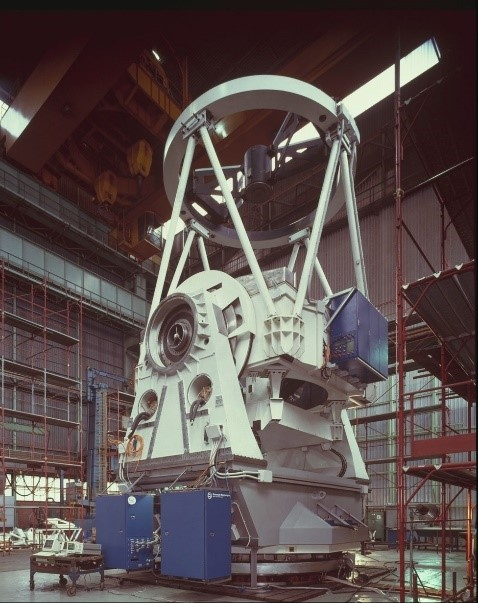
\includegraphics[width=5cm]{11.jpg}
\end{figure}
\end{minipage}
\begin{minipage}{0.5\textwidth}
    \begin{figure}[H]
        \centering
        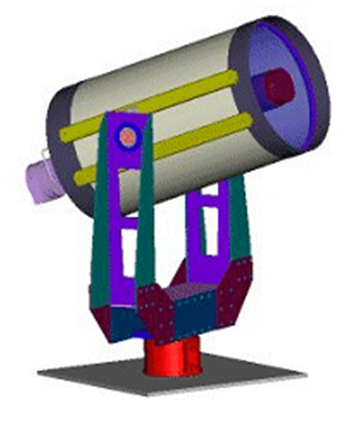
\includegraphics[width=5cm]{immagini/montatura_altazimutale.png}
\end{figure}
\end{minipage}

\vspace{0.2cm}In tale montatura abbiamo:

\begin{itemize}
    \item L'asse di azimut, che segue l'astro da Est ad Ovest;
    \item L'asse di elevazione che eleva il telescopio se l'oggetto osservato si trova ad Est del meridiano e lo abbassa se questo invece si trova ad Ovest;
    \item un cuscinetto posto al fuoco del telescopio che ruota per annullare la rotazione di campo, che è il fenomeno per il quale l'immagine risultante ruota ad una velocità dipendente dalla declinazione del corpo celeste osservato.
\end{itemize}

Man mano che l'oggetto sorge il telescopio si gira verso est, sta quasi in orizzontale e poi, quando l'oggetto culmina, si porta a sud e si alza all'altezza massima dell'oggetto. Con questa montatura si realizzano i più grandi telescopi: a questo punto la montatura è talmente grande che contiene tutti gli strumenti e non solo il telescopio, il cuscinetto in basso ruota, portandosi dietro il telescopio e tutti gli strumenti che sono montati insieme ai telescopi.

\vspace{0.2cm}Risulta importante una proprietà del telescopio che lega il suo diametro alla sua focale, che si chiama \textit{f-number}: esso è un numero che esprime il rapporto focale/diametro ($N=f/D$). Il motivo della sua importanza è che quando i telescopi erano piccoli si poteva andare su f-number molto grandi, cioè focali lunghe e diametri piccoli. Man mano che i telescopi diventano più grandi, la focale non può più essere troppo grande rispetto al diametro, e allora queste focali diventano più corte, tanto corte che possono essere addirittura pari a 1 (se ad esempio il telescopio è dell'ordine di decine di metri, non si può costruire un secondario che sta a 100 metri, lo si deve comunque mettere molto vicino).

\subsubsection{Fuochi di un telescopio}

Parliamo adesso del punto in cui ci posizioniamo o posizioniamo gli strumenti per guardare gli oggetti, cioè i fuochi del telescopio.

Per definizione, il fuoco dello specchio principale, o specchio primario, è il fuoco primario. In una configurazione con un solo specchio, ovviamente, non si possono collocare oggetti molto grandi; purtroppo però con gli anni gli strumenti sono diventati sempre più grandi. Per esempio nella foto l'Anglo Australian Telescope (AAT) ha un fuoco primario che comincia a diventare grande tanto quanto lo specchio primario e quindi non è utile. 

\begin{figure}[H]
        \centering
        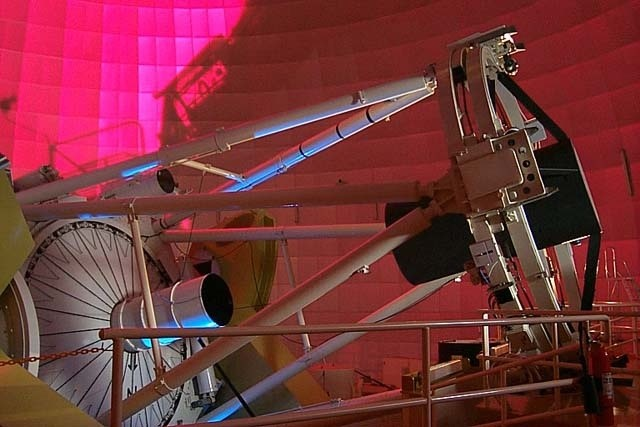
\includegraphics[width=7cm]{12.jpg}
        \label{}
    \end{figure}

Per questo motivo già Newton aveva inventato la collocazione di uno specchio piano che estraesse il fascio focale per la posizione del sensore.

\begin{figure}[H]
        \centering
        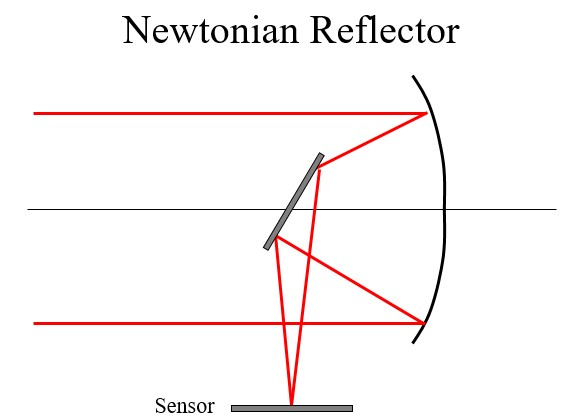
\includegraphics[width=7cm]{13.jpg}
        \label{}
    \end{figure}

Questo tipo di oggetto va bene per piccoli telescopi (cioè non si può immaginare un telescopio newtoniano di grandi dimensioni),

La configurazione che si è affermata nel tempo è la \textbf{Cassegrain}, dove viene posto uno specchio secondario che, sebbene inevitabilmente faccia ombra, ci permetterà di avere un fuoco fisso dove montare lo strumento. Tuttavia, non si può pensare di montare lo strumento sul telescopio perché tutta la struttura risulterebbe troppo pesante (ricordiamo che il telescopio si muove per seguire l'oggetto).
%Tale strumento non può essere montato direttamente al telescopio, in quanto altrimenti quest'ultimo, che si muoverà per seguire gli oggetti, dovrebbe compiere il moto con lo strumento montato (e questo è appunto grande e pesante, può essere pesante quanto un telescopio o forse anche più). Per esempio, a Serra La Nave c'è un telescopio di 1 metro di diametro e lo spettrografo è un banco ottico di 2,4 metri. 
Bisogna allora trovare un modo per trasferire la radiazione dal telescopio allo strumento senza montarlo.

Esistono tante soluzioni: le prime sono state configurazioni un po' più complicate costituite da una serie di specchi che rimandano la luce lungo l'asse di rotazione del telescopio, in cui il primario riflette sul secondario, questo a sua volta riflette su un terziario ed estrae la luce. In questo, comunque il telescopio sia ruotato, qualunque cosa lui guardi, la luce arriva sempre nello stesso punto.

Una configurazione molto utilizzata che permette l'estrazione del fascio è quella in figura:

\begin{figure}[H]
    \centering
    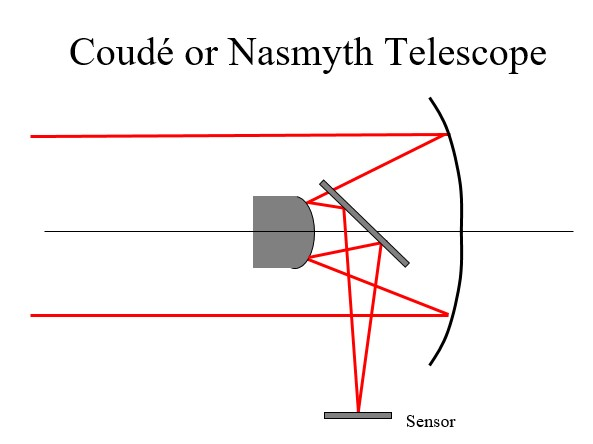
\includegraphics[width=7cm]{14.jpg}
\end{figure}

Essa si chiama configurazione Nasmyth ed è una variante di quella Cassegrain, alla quale viene aggiunto un terzo specchio piano. Nella configurazione Nasmyth lo specchio primario non viene più forato, ma lungo l'asse di declinazione strumentale viene posizionato lo specchio piano (che sta sotto il secondario, quindi non produce ombra) per "estrarre" il fuoco all'interno dell'asse; in tal modo l'immagine va a formarsi all'estremità dell'asse di declinazione dove sono montati gli strumenti di osservazione. Ovviamente si hanno due fuochi (detti fuochi Nasmyth) perché lo specchio sotto può essere girato.

Tutti i grandi telescopi attuali funzionano con questa configurazione. Si tratta, in definitiva, di telescopi alto-azimutali.

Questa è la configurazione finale dei telescopi attuali.

\subsubsection{Il processo di "coating"}
Vediamo in dettaglio come rendere riflettente una superficie. Il processo adoperato per le lenti dei telescopi si chiama \textit{coating} o deposizione: si prende lo specchio di vetro e lo si deposita all'interno di una struttura come quella in foto che prende il nome di campana, che è un luogo dove si può creare il vuoto.

\begin{minipage}{0.395\textwidth}
    \begin{figure}[H]
        \centering
        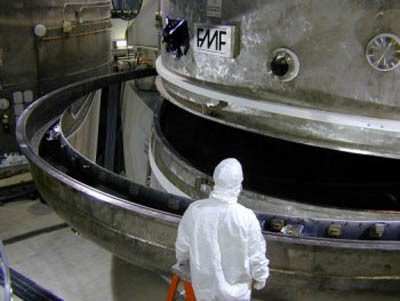
\includegraphics[width=6cm]{15.jpg}
    \end{figure}
\end{minipage}
\begin{minipage}{0.6\textwidth}
    \vspace{0.3cm}Dopo aver sigillato e creato il vuoto con delle pompe, è possibile far evaporare all'interno, per esempio, dell'alluminio. L'alluminio diventa un gas, riempie l'intera campana e quando si raffredda si deposita creando un coating, un deposito di alluminio sul vetro. Il motivo per cui eseguiamo proprio questa procedura è che con essa possiamo sapere esattamente qual è lo spessore di alluminio e sappiamo che l'alluminio si depositerà in maniera omogenea, conservando la forma iniziale dello specchio.
\end{minipage}

\vspace{0.2cm}Qual è la capacità di riflettere la luce dell'alluminio?

Osserviamo il grafico di seguito rappresentato: nella foto l'alluminio è la curva verde:

\begin{minipage}{0.495\textwidth}
    \begin{figure}[H]
        \centering
        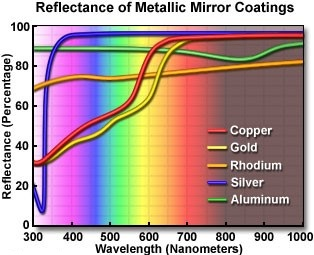
\includegraphics[width=7cm]{16.jpg}
    \end{figure}
\end{minipage}
\begin{minipage}{0.5\textwidth}
    \vspace{0.5cm}Dal grafico si evince che non siamo in grado di produrre una riflettività del 100\%, tuttavia l'alluminio è uno dei materiali più utilizzati perché è di basso costo, inoltre costituisce un buon compromesso per avere una buona riflettività su tutto, sebbene abbia riflettività solo del 90\%. Bisogna fare attenzione al fatto che ogni volta che mettiamo uno specchio perdiamo il 10\% di riflettività.
\end{minipage}

\vspace{0.2cm}L'alluminio però ha un problema: dopo un po' diventa opaco, quindi va tolto e rimesso, fatto che non avviene con altri materiali. Potremmo allora pensare di realizzare, ad esempio, un deposito di oro, ma in questo caso avremmo che, poiché la riflettività risulta essere una funzione della lunghezza d'onda, quest'ultima sarebbe molto alta nell'infrarosso e poco invece nella luce visibile (curva gialla).


 
\subsubsection{Uso degli attuatori}
%Dunque per fare un telescopio bisogna prestare attenzione a dei fattori. Come si fa a far sì che funzioni nella realtà? Quando io costruisco un oggetto, questo si piega (ora magari non è tanto, perché è un oggetto rigido come uno specchio, però quel poco può essere un problema. Inoltre gli assi delle due coniche devono avere i fuochi coincidenti; se l'asse un po' si sposta significa che non va più a fuoco).
I telescopi hanno bisogno di una struttura che non solo permetta di farli girare, ma che garantisca anche la qualità dell'ottica. Ciò non è facilmente ottenibile quando gli strumenti diventano grandi: lo specchio in vetro, anche se è perfetto, non manterrà la sua forma (soprattutto a terra con la gravità). Si è pensato allora di costruire non più specchi tanto spessi, in grado di sostenere la gravità da soli, ma piuttosto specchi di vetro sottile (non più di 20 cm), che vanno poi posti su una struttura di metallo. In questa struttura di metallo ci saranno degli attuatori (pistoni) che possono spingere o tirare, quindi quando il telescopio punta qualcosa, se si deforma, si tireranno gli attuatori giusti e si spingeranno gli altri affinché il telescopio abbia la forma ottimale. Stiamo quindi parlando di \textbf{ottica attiva}.

%Questo è l'unico modo per avere i telescopi effettivamente sempre ben allineati;
Tale metodo viene adoperato anche in un telescopio a mosaico, dove gli specchi sono montati su attuatori. In pratica si punta un oggetto, si fa un'analisi dell'immagine e si dà una forma agli specchi (muovendoli con gli attuatori) affinché l'immagine venga corretta. È una cosa che si può fare facilmente perché esiste un'analisi del fronte d'onda (mediante Polinomi di Zernike), che dice come bisogna muovere gli attuatori perché lo specchio abbia la forma ideale. Così è costruito il TNG, ma oggi si va ad un passo successivo, in cui anche il secondario è attivo.

%Quindi, in pratica, io cambio queste cose fino a che non trovo la posizione ottimale degli specchi per avere le immagini al meglio.


\begin{minipage}{0.5\textwidth}
    \begin{figure}[H]
        \centering
        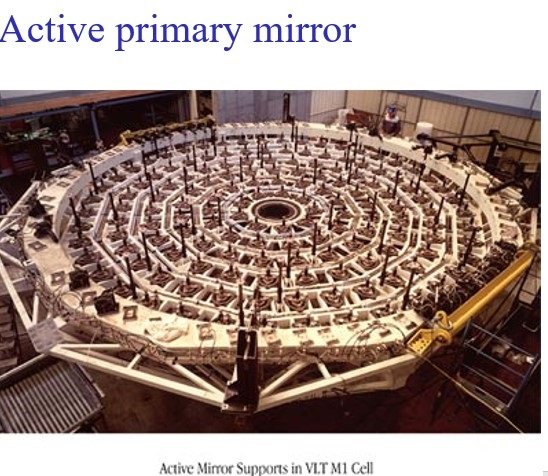
\includegraphics[width=7cm]{17.jpg}
\end{figure}
\end{minipage}
\begin{minipage}{0.5\textwidth}
    \begin{figure}[H]
        \centering
        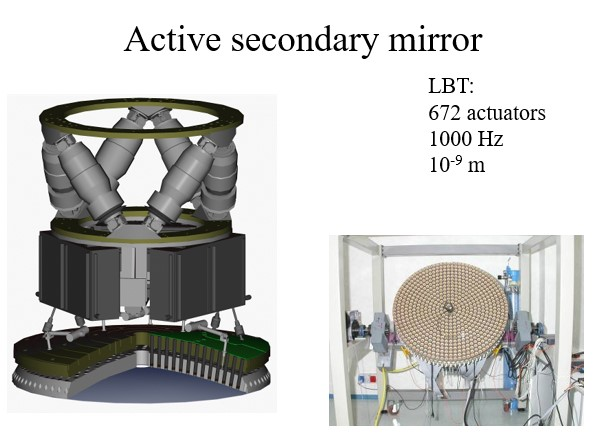
\includegraphics[width=7cm]{18.jpg}
    \end{figure}
\end{minipage}

\subsubsection{Il ruolo dell'atmosfera nell'osservazione, il "seeing" e l'ottica adattiva}
Prima di arrivare sul telescopio, la radiazione proveniente dalle stelle avrà attraversato l'intera atmosfera, venendo alterata. Ne segue che l'idea che l'immagine di una sorgente puntiforme sia determinata dalla dimensione del telescopio potrebbe non essere più vera.

Quello che nella pratica succede è che, immaginando che l'atmosfera sia fatta a strati, man mano che la radiazione incontra questi vari strati caratterizzati da un indice di rifrazione diverso da 1, questa subisce uno spostamento spaziale (viene variata la direzione). Il risultato finale per l'osservatore è che la stella sembra muoversi\footnote{Questo lo percepiamo anche quando guardiamo il cielo: i pianeti sembrano fissi, le stelle sembrano luccicare.}.

Concettualmente questo fatto è uguale alla matita nel bicchiere che si spezza, ma si può anche vedere in un altro modo un po' più sofisticato.

\begin{figure}[H]
    \centering
    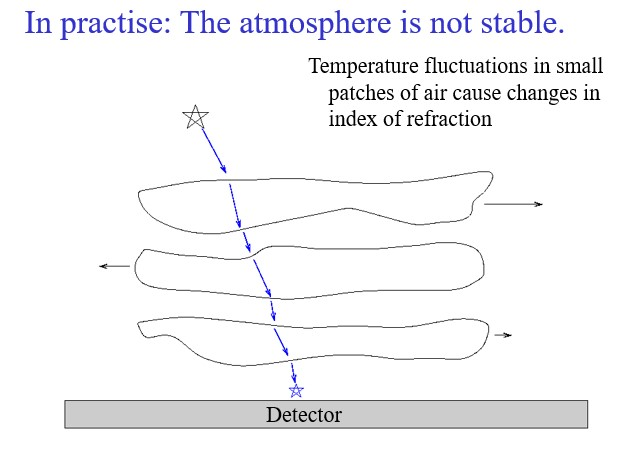
\includegraphics[width=9cm]{19.jpg}
    \label{}
\end{figure}

Ribadendo ancora il concetto, l'atmosfera è in grado di aberrare l'immagine, per cui un'immagine, per esempio, perde i contorni. Il ruolo dell'atmosfera è quindi quello di vanificare l'idea che le dimensioni di una sorgente siano assegnate solo dal diametro dello specchio, perché il fronte d'onda piano che attraversa l'atmosfera incontra celle dall'indice di rifrazione diverso (lo abbiamo visualizzato come se fosse tutto uno strato che cambia, però nella realtà, ogni porzione dell'atmosfera ha un proprio indice di rifrazione). Quindi, sul piano focale, in realtà, non si forma una sola immagine ma se ne formano tante, una per ogni colonna d'aria; il risultato è che sul fondo si formano tante immagini diverse che noi percepiamo come un allargamento dell'immagine e una perdita dei contorni. Questo accade per ogni colonna, e ognuna di queste cambia in continuazione le sue proprietà. \E chiaro che la qualità dell'immagine dipende dal cielo: se guardiamo una stella al livello del mare appare in un modo; man mano che si sale di quota si riduce la colonna d'aria e l'immagine appare migliore; questo è il motivo per cui i telescopi si montano tutti ad altezze elevate. Questo effetto si chiama \textit{seeing} ed è quello che in realtà dà la dimensione alle immagini delle stelle.

Nota: l'altezza della colonna d'aria in cui i parametri dell'atmosfera restano costanti dipende dalla lunghezza d'onda. Quando parliamo di luce visibile si parla di 10 cm, mentre quando andiamo nell'infrarosso questa colonna d'aria è grande 8 metri, quindi gli effetti sono molto diversi sul telescopio. Se andiamo invece nel radio, la colonna d'aria in cui il fronte d'onda non cambia è di 15 km, quindi non ci sono tanti problemi.

\begin{figure}[H]
    \centering
    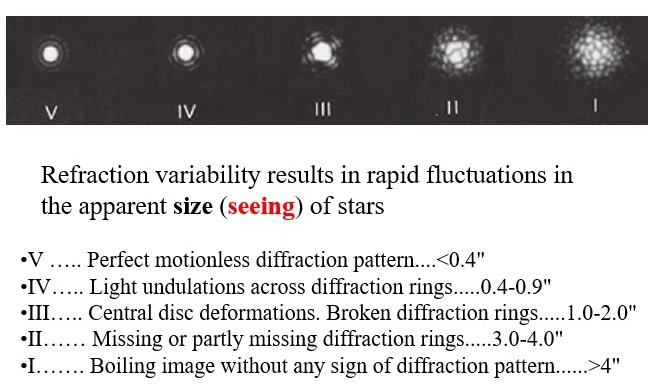
\includegraphics[width=9cm]{20.jpg}
\end{figure}

Il seeing non rappresenta un gran problema per gli oggetti puntiformi perché, in fondo, non è cambiata la quantità di energia che è arrivata a Terra (è sempre la stessa, solo sparpagliata); ad esempio una stella sul livello del mare appare come 5 arcsec, mentre in un posto buono può essere 0.15 arcsec. Il seeing, che abbiamo detto costituisce un allargamento dell'immagine, diventa però fastidioso quando consideriamo oggetti estesi, perché si perde il contorno.

Il seeing è definito come la lunghezza d'onda diviso il parametro di Fried $r_0$, cioè il diametro della colonna d'aria in cui non si osserva variazione:

\begin{equation}
    \Delta\theta=\frac{\lambda}{r_0}
\end{equation}

Come risolviamo il problema?

Consideriamo un fronte d'onda istantaneo come in figura:

\begin{figure}[H]
    \centering
    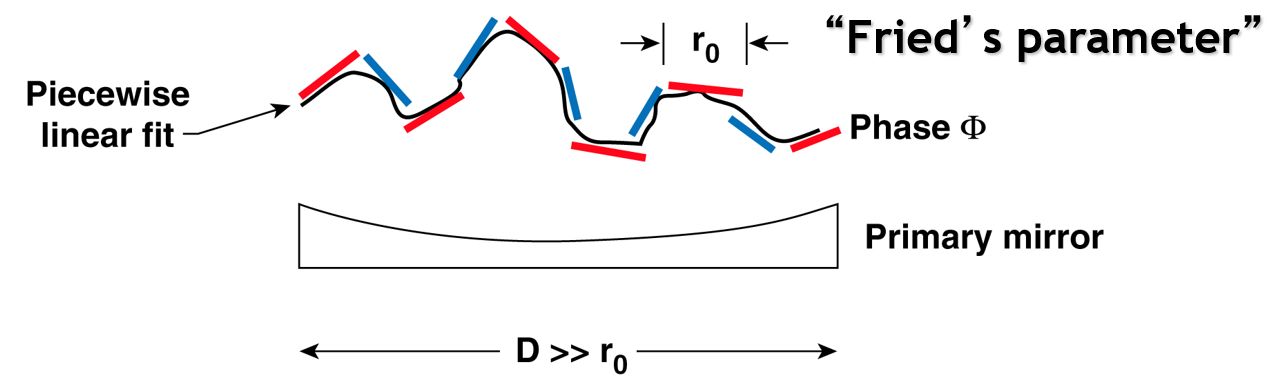
\includegraphics[width=11cm]{immagini/tempo_di_coerenza.png}
\end{figure}

L'onda resterà tale per un certo intervallo di tempo detto \textit{tempo di coerenza} $t_0$ (della durata di 1 centesimo di secondo). Durante il tempo di coerenza vengono eseguite le seguenti operazioni (illustrate in figura):

\begin{minipage}{0.5\textwidth}
    \begin{figure}[H]
        \centering
        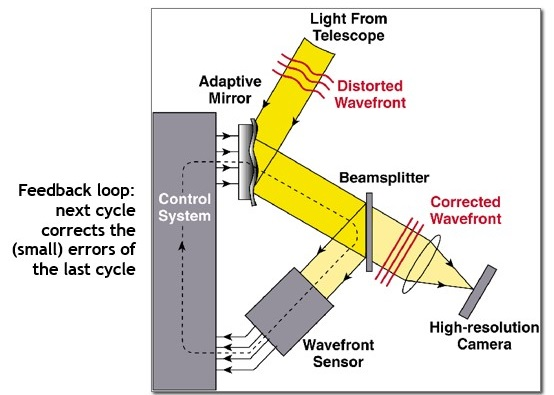
\includegraphics[width=8cm]{21.jpg}
    \end{figure}
\end{minipage}
\begin{minipage}{0.5\textwidth}
    \begin{figure}[H]
        \centering
        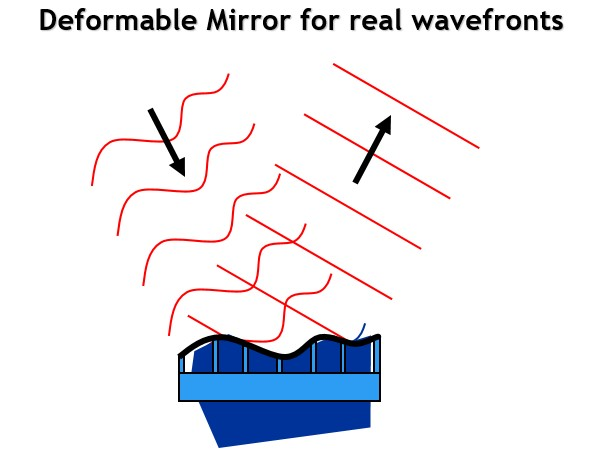
\includegraphics[width=6cm]{22.jpg}
    \end{figure}
\end{minipage}

\begin{enumerate}
    \item Si fa incidere la luce su uno specchio deformabile (a cui possiamo dare la forma che vogliamo, in quanto costituito da un centinaio di attuatori, per cui è detto \textit{adattivo});
    \item Si fa attraversare la luce per uno specchio, detto Beamsplitter o semiriflettente, che fa passare tutta la luce tranne un po' (circa il 10\%), per poi mandarla verso il sensore;
    \item Si analizza la parte riflessa per scoprire come il fronte d'onda è stato deformato dall'atmosfera, in modo da capire che configurazione deve assumere lo specchio affinché si compensi la deformazione, così da riottenere un fronte d'onda piano.
\end{enumerate}

Nelle seguenti figure possiamo vedere l'immagine osservata al telescopio prima e dopo aver applicato l'ottica adattiva:

\begin{minipage}{0.5\textwidth}
    \begin{figure}[H]
        \centering
        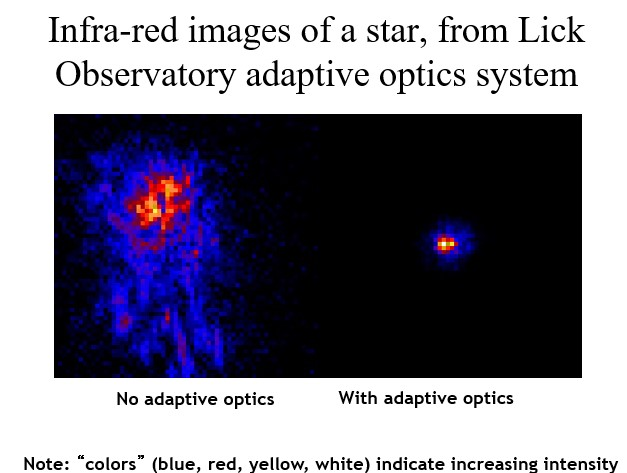
\includegraphics[width=8cm]{23.jpg}
    \end{figure}    
\end{minipage}
\begin{minipage}{0.5\textwidth}
    \begin{figure}[H]
        \centering
        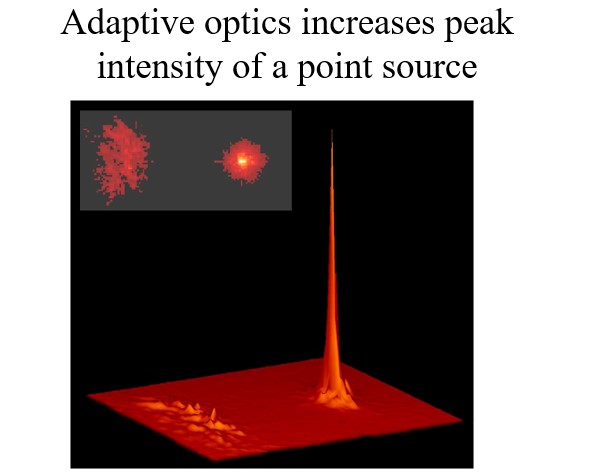
\includegraphics[width=8cm]{24.jpg}
    \end{figure}
\end{minipage}

\vspace{0.2cm}L'ottica adattiva si può applicare quando è possibile estrarre un po' di luce e fare l'analisi del fronte d'onda, ma questa prevede che si abbiano dei fotoni, quindi l'oggetto deve essere brillante abbastanza brillante. Se stiamo studiando una stella più debole della decima, potremmo analizzare una stella vicina (non è necessario fare l'analisi del fronte d'onda esattamente sulla stessa stella).

A volte succede che tale stella non c'è; in questi casi basta avere associato al nostro telescopio un laser: sostanzialmente quello che si fa è sparare con un laser nella direzione di osservazione. A 92 km dal mare in altezza abbiamo uno strato di sodio e il laser lo incontra. La frequenza del laser è esattamente la frequenza necessaria per creare una transizione atomica nel sodio. Infatti gli elettroni passano da un livello a un altro se colpiti da un fotone opportuno; questo fotone, che è il nostro laser, con una lunghezza d'onda di 590 nm, trasferisce gli elettroni del sodio da un livello a un altro. L'elettrone non può però stare in uno stato eccitato, quindi decade e riemette un fotone. Il fotone, questa volta, viaggerà verso il telescopio e farà lo stesso percorso della luce della stella; in questo modo costruiamo una "stella digitale" vicino a quella reale, di cui analizziamo il fronte d'onda distorto. Uno dei sistemi attuali prevede che la stella reale sia accerchiata da 4 stelle artificiali, in modo da poter fare delle correzioni angolari (perché ci sono delle differenze: se guardiamo in una direzione il fronte d'onda si deforma in un modo, se guardiamo in un'altra si deforma in un altro modo). Esiste un angolo, detto \textit{isoplanatico}, definito come l'angolo entro cui possiamo spaziare senza che il fronte d'onda sia pià aberrato di $r_0$.
 
\subsubsection{L'atmosfera come un prisma}
L'atmosfera si comporta come un prisma, in quanto ha un indice di rifrazione $n$, il quale dipende dalla lunghezza d'onda ed è dato da

$$n=1 + 7.76 \cdot 10^{-5} K mb^{-1} \left( \frac{P_d}{T} \right) - 5.6 \cdot 10^{-6} K mb^{-1} \left( \frac{e}{T} \right) + 0.375 K^2 mb^{-1} \left( \frac{e}{T^2} \right)$$

dove il primo termine dipende dalla densità dell'aria, che è funzione della pressione $P_d$ dell'aria, e della temperatura $T$; gli altri due dalla temperatura e dalla pressione di vapore $e$.

Essa ci dice che $n$ cambia con la pressione e con la temperatura, quindi non si può prevedere. Per dare un'idea degli ordini di grandezza, sul livello del mare $n=1.003$ e nello spazio $n=1.000$.

%\begin{figure}[H]
%        \centering
%        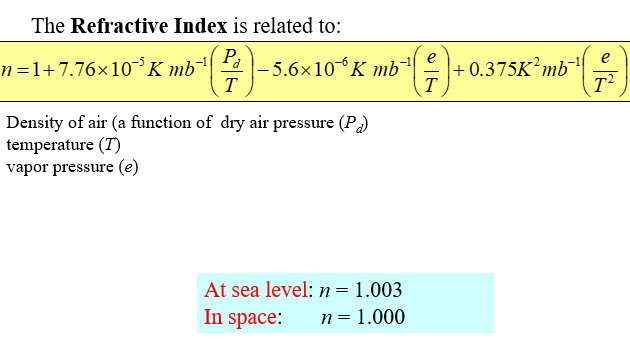
\includegraphics[width=9cm]{25.jpg}
%        \label{}
%    \end{figure}

La rifrazione causa un cambio di percorso nella radiazione, per cui pone due problemi. Un primo problema è che le stelle non sono dove sembrano stare apparentemente, per cui non sappiamo dove puntare il telescopio se non a posteriori; il secondo problema è che l'atmosfera, comportandosi come un prisma, scompone la stella nei suoi colori:

\begin{minipage}{0.5\textwidth}
    \begin{figure}[H]
        \centering
        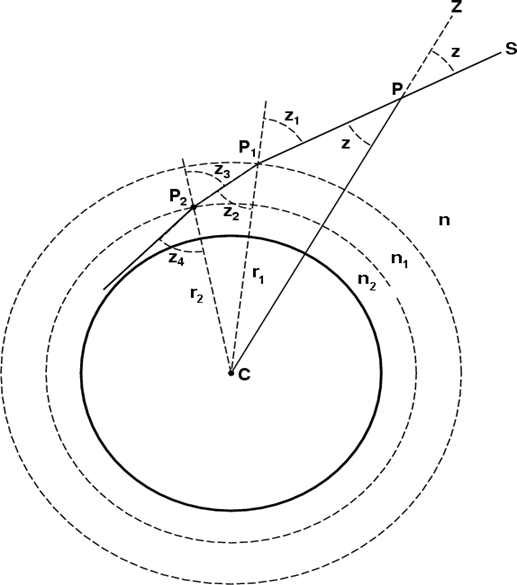
\includegraphics[width=4cm]{immagini/legge_di_snell.png}
    \end{figure}
\end{minipage}
\begin{minipage}{0.5\textwidth}
    \begin{figure}[H]
        \centering
        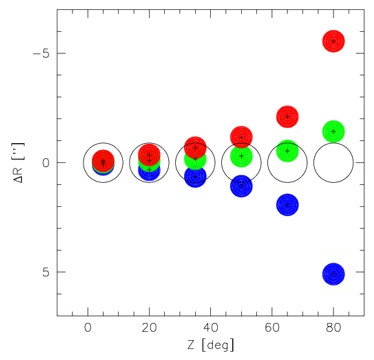
\includegraphics[width=5cm]{immagini/spostamento_colori_atmosfera.png}
    \end{figure}
\end{minipage}

\vspace{0.2cm}Dalla legge di Snell sappiamo che nel caso in cui la radiazione incida perpendicolarmente all'atmosfera, non ci sarà spostamento dell'immagine: tutti i colori saranno perfettamente sovrapposti; man mano che ci spostiamo in distanza zenitale la luce comincia a piegare apparentemente in maniera diversa a seconda della lunghezza d'onda, per cui abbiamo variazioni (quando l'oggetto è molto basso) che sono dell'ordine di 10 arcsec. Questo significa che la stella apparirà come un cerchio allungato nella direzione verticale.

\subsubsection{Potere risolutivo di un telescopio}
Abbiamo parlato finora di telescopi, cioè di un oggetto che sostanzialmente è una fenditura circolare che raccoglie la radiazione (l'onda piana prodotta dagli oggetti), dando origine sul piano focale a una figura definita dalla Point Spread Function e che per le lenti circolari si chiama “disco di Airy”, dal signore che lo ha battezzato, costituita da una serie di anelli concentrici. Esso ha una posizione, il primo zero, che è legato al diametro del foro di un telescopio.

\begin{figure}[H]
    \centering
    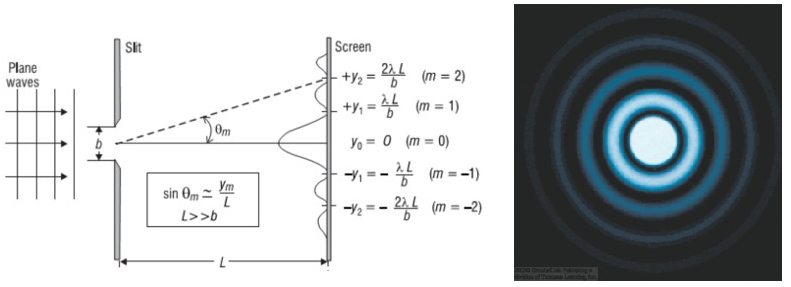
\includegraphics[width=12cm]{immagini/interferometria_1.png}
\end{figure}

Esiste un modo di aumentare il potere risolutivo dei telescopi (perché di fatto questo limita la nostra capacità; un oggetto più piccolo del disco di Airy noi non lo possiamo vedere come risolto)?

Esiste la possibilità di farlo, e si basa sull'interferometria, che si basa sull'esperimento delle due fenditure. Immaginiamo di avere due telescopi che guardano entrambi nella medesima direzione:

\begin{minipage}{0.5\textwidth}
    \begin{figure}[H]
        \centering
        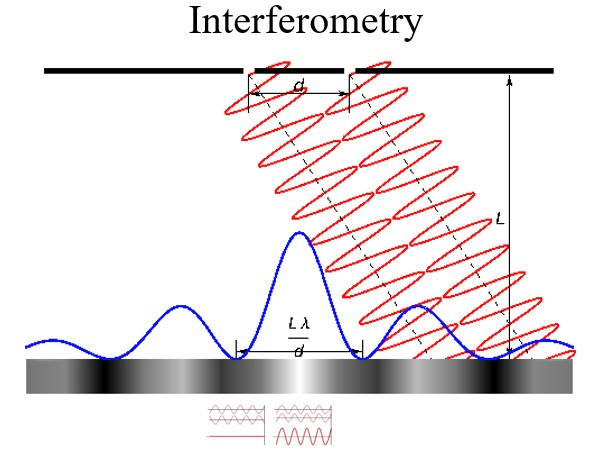
\includegraphics[width=7cm]{28.jpg}
    \end{figure}
\end{minipage}
\begin{minipage}{0.5\textwidth}
    \begin{figure}[H]
        \centering
        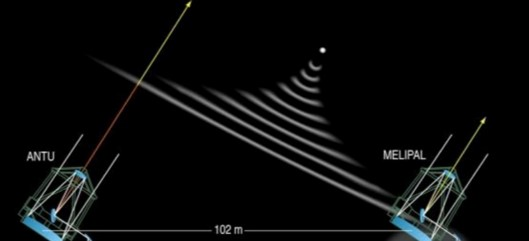
\includegraphics[width=7cm]{29.jpg}
    \end{figure}
\end{minipage}

Quello che succederà, ovviamente, è che uno dei due telescopi vedrà arrivare il fascio di luce un po' prima dell'altro, quindi non saranno più in fase. Se però attuiamo una correzione della fase, si può dare origine a una figura di interferenza. In questo modo possiamo realizzare le frange di interferenza così come le fanno due fenditure. Questa volta, però, lo zero non è più in relazione con il diametro del telescopio, bensì con la distanza dei due telescopi che può essere, per esempio, dell'ordine di 100 metri, quindi si può avere un potere risolutivo che è 10 volte maggiore (rispetto a quello dato da un singolo telescopio di 10 metri).

Il problema di questo metodo è che la risoluzione angolare viene aumentata soltanto lungo la direzione della congiungente i due telescopi, mentre in tutte le altre sarà data da quella del singolo specchio. Per ovviare al problema si può pensare di usare più di due telescopi, ed è quello che si è fatto con il Very Large Telescope Interferometer (VLTI) che prevede 4 telescopi di 8 metri più una batteria di telescopi piccoli.

\begin{figure}[H]
    \centering
    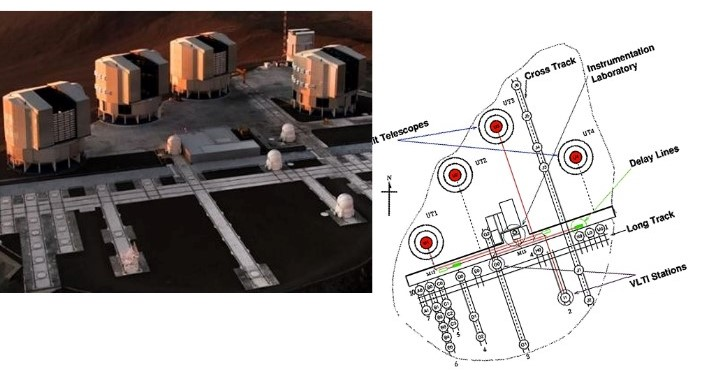
\includegraphics[width=8cm]{30.jpg}
\end{figure}

Tutti i telescopi guardano il medesimo oggetto e per ogni coppia di telescopi si crea una figura di interferenza. Unendo tutte le figure di interferenza si può realizzare un'immagine che è effettivamente molto risolta in tutte le direzioni angolari.

\subsubsection{Radio telescopi}
\E possibile osservare non solo con telescopi ottici, ma anche con telescopi radio (in foto il Telescopio di Noto).

\begin{figure}[H]
    \centering
    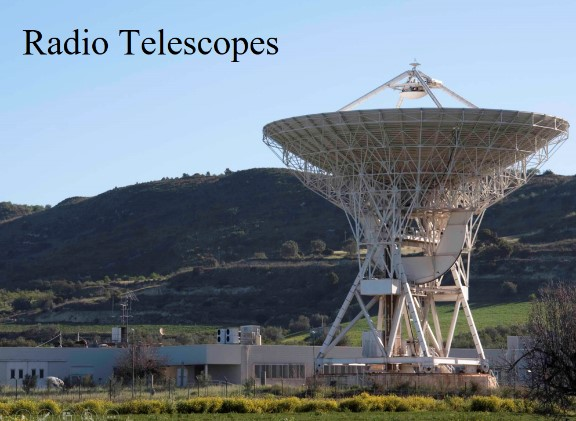
\includegraphics[width=7cm]{31.jpg}
\end{figure}

I telescopi radio non sono molto diversi da quelli ottici: anch'essi hanno una montatura alto-azimutale e un focal number molto corto, perché la larghezza del telescopio non è molto diversa dalla focale. Il telescopio ha un fuoco primario su cui sono poggiati una serie strumenti (nel caso radio si parla di ricevitori) e questi telescopi radio sono molto simili a quelli ottici più grandi. Allo stato attuale, i telescopi radio più grandi al mondo sono “Green Bank” negli Stati Uniti con 43 metri e “Effelsberg” a Bonn di 100 metri, “Arecibo” di 300 metri che ha una caratteristica molto diversa: questo non si può orientare, osserva ciò che passa (il telescopio “Arecibo” è stato dismesso qualche anno fa ed è stato sostituito da questo telescopio cinese che si chiama “FAST” di 500 metri). 

\begin{figure}[H]
    \centering
    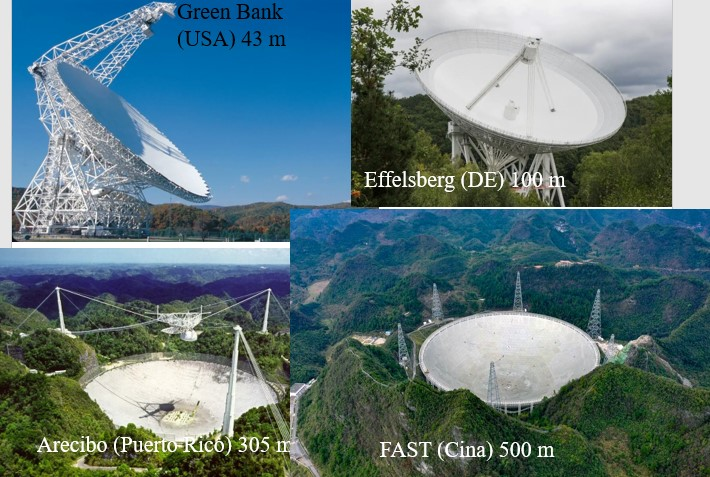
\includegraphics[width=7cm]{32.jpg}
\end{figure}

I singoli telescopi in radioastronomia non hanno grande fortuna, perché parliamo di lunghezze d'onda dell'ordine decine di centimetri e, anche nel radiotelescopio, vale la regola per cui la funzione di interferenza al primo fuoco vale $1.22 \cdot {\lambda}/d$, ma ${\lambda}$ vale centimetri questa volta, per cui nel radio l'interferometria è la tecnica maggiormente utilizzata.

Il radiotelescopio così costruito diventa però un interferometro con una base di 27 km. Si ottiene dunque un potere risolutivo superiore a quello di quelli ottici. Il futuro degli interferometri si chiama “Square Kilometer Array (SKA)”: si parla di centinaia di telescopi che riempiranno l'Australia (costa ovest) e avranno una superficie di rapporto equivalente 1 km. 

\begin{figure}[H]
    \centering
    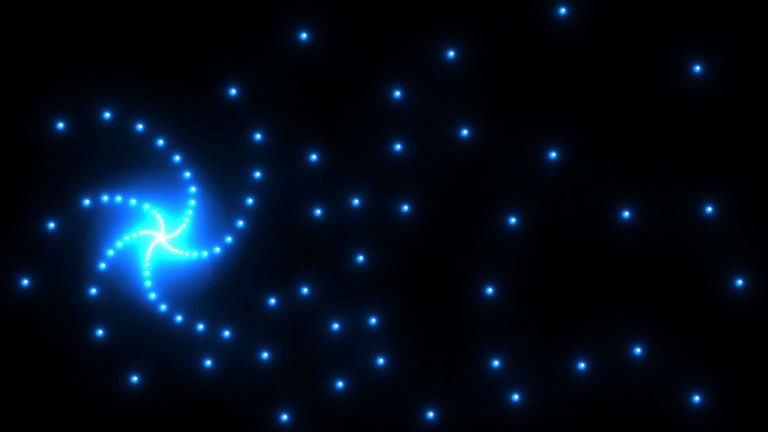
\includegraphics[width=7cm]{33.jpg}
\end{figure}

Il più famoso interferometro è quello che ha visualizzato il buco nero al centro della galassia di M87. Questo è un array di telescopi che è distribuito su tutta la superficie della Terra. Sono state combinate le misure di varie antenne (una sta al Polo Sud, una in Danimarca, una vicino alle Hawaii, ecc.) Tutti questi hanno combinato i loro segnali per produrre un'immagine di quello che dovrebbe essere l'ambiente che circonda il buco nero (non è stata fatta la foto del buco nero, ma dell'ambiente che lo circonda). Queste misure sono fatte non nel centimetrico, bensì a 1.3 mm (230 GHz).

\begin{figure}[H]
    \centering
    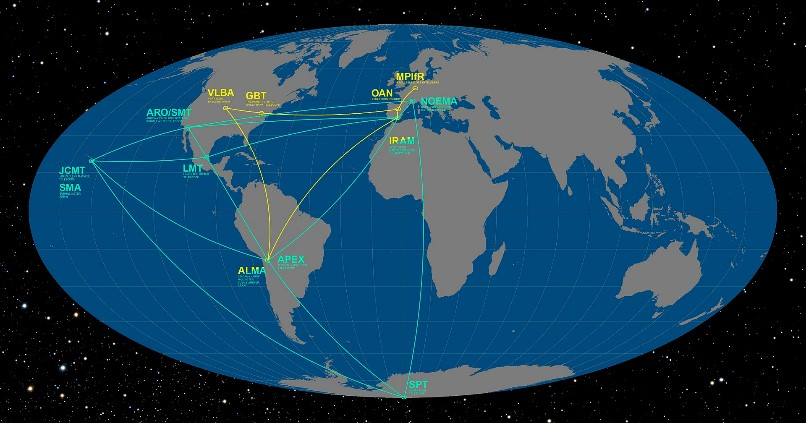
\includegraphics[width=7cm]{34.jpg}
\end{figure}

Nota: i telescopi prendono i dati a coppie. 
I radioastronomi, rispetto ai solari non hanno il problema del maltempo, perché le onde passano (la televisione si vede anche se piove). La visibilità dell'oggetto può non essere simultanea per tutti i telescopi. L'Italia è al momento impegnata nella realizzazione del primo strumento dove il ricevitore è bidimensionale: cioè, finora il radio aveva una sola antenna e vedeva un posto solo; questo sarà un ricevitore bidimensionale e potrà fare un'immagine di tutto il cielo contemporaneamente. Bisogna solo decidere cosa vedere perché è troppa l'informazione che arriva.

Ma qual è il vantaggio del radio rispetto all'ottico? Le onde radio, rispetto all'ottico, hanno il vantaggio di non essere fermate dalla materia. Questo vuol dire che le onde radio sono in grado di propagarsi attraverso la materia dello spazio, quindi possiamo vedere per esempio il centro della galassia che è invisibile all'ottico perché la luce, la radiazione visibile, che parte dal centro della galassia, viene fermata dalla materia che la circonda. Quindi il radio ha il vantaggio di farci vedere più lontano rispetto all'ottico.

\subsection{UV, infrarosso, X}

Abbiamo affrontato i visibile e poi il radio, che da un punto di vista strumentale è identico al visibile. Non possiamo invece vedere da Terra né l'ultravioletto, né l'X, perché interviene l'assorbimento dell'atmosfera (vedi la curva di trasmissione nella figura).

\begin{figure}[H]
    \centering
    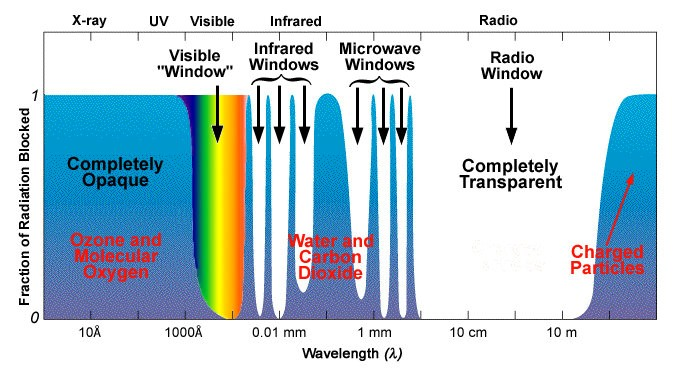
\includegraphics[width=10cm]{35.jpg}
\end{figure}

Per queste bisogna fare delle osservazioni spaziali, sebbene abbiamo comunque una tecnologia per l'ultravioletto e l'infrarosso identica a quella dei telescopi a terra.

Quelli che invece hanno un po' di differenza sono i cosiddetti “Telescopi X”. I raggi X attraversano la materia, quindi non è facile intercettarli; l'idea allora è stata di utilizzare una riflessione radente: i telescopi X, che sono nello spazio, sono costituiti da una superficie curva che è una porzione di paraboloide, seguito da una superficie curva che è un iperboloide, per correggere e convogliare la radiazione sul sensore. Siccome non è possibile fare oggetti molto grandi, si è pensato di aumentare la superficie di raccolta con una serie di telescopi concentrici uno all'interno dell'altro. È così che è stato realizzato il telescopio più famoso che è “Chandra” e che è in orbita.

\begin{minipage}{0.5\textwidth}
    \begin{figure}[H]
        \centering
        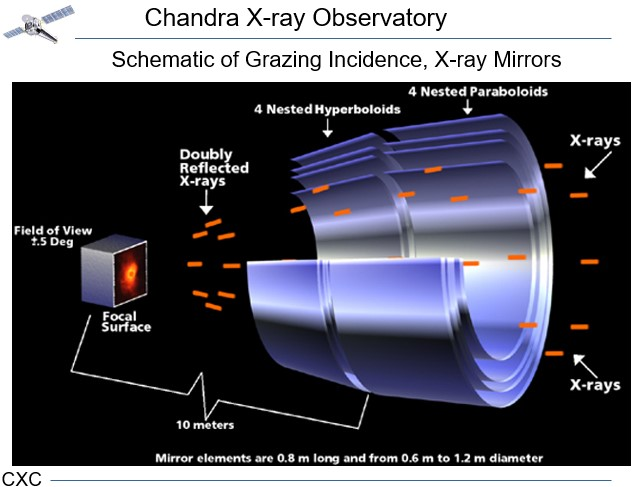
\includegraphics[width=7cm]{36.jpg}
    \end{figure}
\end{minipage}
\begin{minipage}{0.5\textwidth}
    \begin{figure}[H]
        \centering
        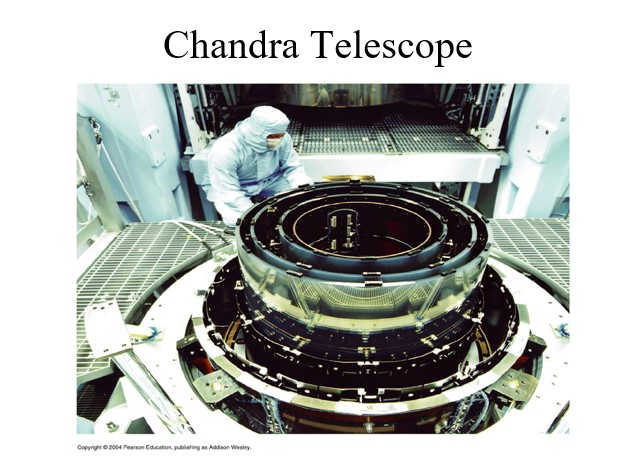
\includegraphics[width=7cm]{37.jpg}
    \end{figure}
\end{minipage}

\vspace{0.2cm}Per la tecnologia degli X nel 2002 è stato premiato con il Nobel il prof. Riccardo Giacconi.

\subsection{I gamma}

Rimane l'ultima parte dello spettro, che sono i gamma. È la parte tipica dell'alta energia.

Un fotone gamma si produce sostanzialmente in due modi:

\begin{enumerate}
    \item Un modo è per Compton inverso, in cui si ha un elettrone relativistico che colpisce un fotone normale (infrarosso normalmente) e gli cede la propria energia, quindi il fotone diventa altamente energetico.
    
    Vediamo più nel dettaglio: esiste un fenomeno che si chiama Effetto Compton secondo cui un fotone può cedere la propria energia a una particella. Esiste anche la probabilità di avere il processo inverso, che si chiama Compton inverso: il Compton inverso prevede che un elettrone relativistico molto energetico, collida con un fotone e ceda al fotone la sua energia, cioè significa cambiarne la frequenza (la velocità è sempre $c$, non può cambiare, però la sua frequenza può crescere e passare dal visibile/infrarosso al gamma);
    \item Un'altra possibilità è invece di produrre gamma nelle reazioni nucleari.
\end{enumerate}

I raggi gamma vengono osservati con degli scintillatori (montati sui satelliti), materiali che se attraversati da gamma producono fotoni, i quali vengono poi "amplificati" da dei fotomoltiplicatori che servono ad amplificare il segnale iniziale.

\begin{figure}[H]
    \centering
    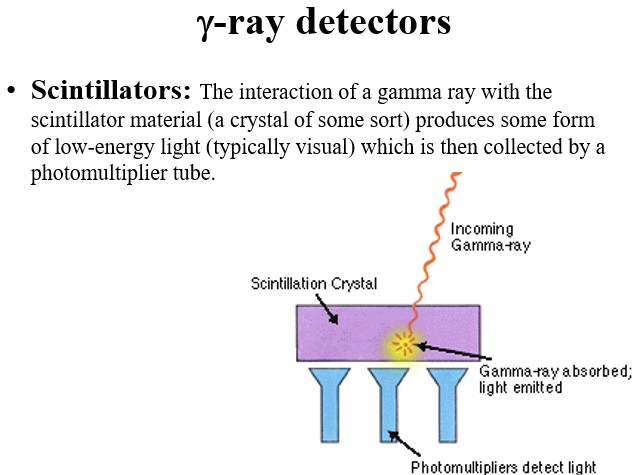
\includegraphics[width=8cm]{38.jpg}
\end{figure}

I fotoni gamma, che non arrivano a Terra, si possono vedere anche con i telescopi. Questo perché a terra succede che una particella che arriva ad alte energie dall'atmosfera produce una cascata di particelle (sciame).Tale sciame è fatto di particelle che hanno una velocità superiore alla velocità della luce in aria, quindi producono radiazione Cherenkov\footnote{Se abbiamo una particella carica che si muove dentro un mezzo ad una velocità superiore alla velocità della luce, le molecole, gli atomi di questo ambiente vengono polarizzate al passaggio della carica elettrica. Quando poi ritornano alla configurazione iniziale, emettono un bagliore, che è stato appunto dedicato a Cherenkov e viene chiamato oggi luce Cherenkov. Lo scopritore restò chiuso in una stanza molto buia per vedere l'emissione che particelle dalla velocità superiore alla velocità della luce nel mezzo producevano.}; propagandosi lo sciame illumina il terreno con un cono di luce che è nel visibile (va da 400 a 800 nm. Lo stesso vale in acqua: in acqua è stata sfruttata la luce Cherenkov, cioè particelle veloci in acqua, per la detection dei neutrini del Sole ad esempio), il quale dura 5 ns su 10 fotoni al metro quadrato, noi mettiamo dentro un telescopio e guardiamo la luce che viene prodotta dal Cherenkov. In questo modo, se mettiamo più di un telescopio , riusciamo esattamente a capire da che direzione è arrivato il gamma. Questi Cherenkov Telescope sono telescopi normalmente creati con mosaici di specchi, sono di dimensioni molto grandi, non hanno una grande qualità ottica e di telescopi Cherenkov nel mondo ne esistono 4 array, perché da solo non basta, serve un insieme.
L'INAF ne ha due grandi alle Canarie, poi ne abbiamo uno negli Stati Uniti che si chiama Veritas, un array che sta in Namibia si chiama H.E.S.S. dedicato a Hess che ha scoperto i raggi cosmici e poi ne abbiamo uno in Australia (che non è molto efficiente). Quindi sostanzialmente possiamo fare una misura dell'emissione di raggi gamma usando anche telescopi tradizionali.

Tutto questo perché, come dicevamo prima, una sorgente dobbiamo guardarla da gamma al radio 

\begin{figure}[H]
    \centering
    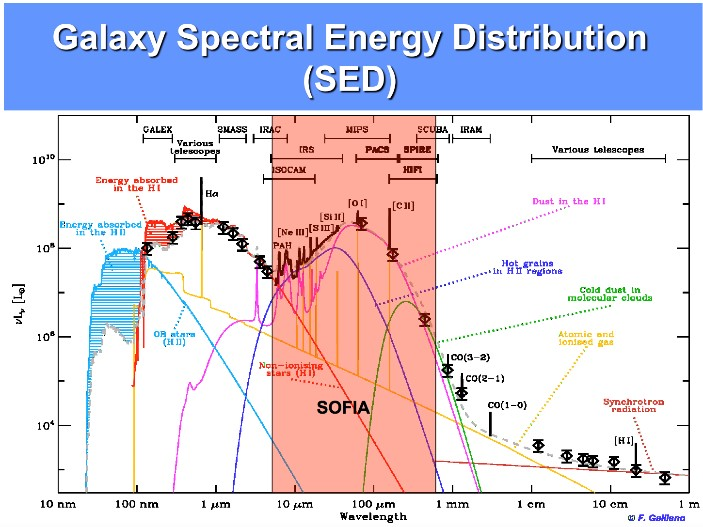
\includegraphics[width=10cm]{39.jpg}
\end{figure}

(In figura: Distribuzione in energia di una galassia.)

Questo è il concetto moderno di astronomia, in cui si deve essere in grado di comprendere i processi fisici che ci sono dietro ogni tipo di emissione: per esempio, per una Galassia bisogna chiedersi come è fatta per spiegare tutte le parti che vediamo.